\chapter*{Моё решение (Прянишников Александр)}


\subsection*{Целевая переменная}
Первое, что меня смутило: задача состоит в прогнозировании \textbf{сдачи} теста, в то время как в программе в качестве целевой переменной используется тестовый балл. 
С одной стороны да, мы можем точнее оценить потенциал ученика. 
Но с другой стороны, даже в первых пяти записях видно, что под индексами 2 и 4 ученики абсолютно идентичны, но у одного target = 1, у другого - 0. 
Также видно, что человек с 79 баллами за тест не сдал, в то время как с 72 и 77 сдали. (И это только head()!)

Тут есть несколько вариантов. 
Первое - выборка была собрана с ошибками, тогда вообще теряется смысл что-то по ней предсказывать. 
Но я оптимист - считаю, что данные +- корректны, и дальше буду этого придерживаться. 
Поэтому нужно сказать, что в таком случае posttest - это не целевая переменная, так как от неё напрямую не следует то, что был факт сдачи экзамена, поэтому логичнее бы было делать целевой переменной target.

\subsection*{Предобработка данных}
Затем, сразу видно столбцы "Unnamed: 0" и "Unnamed: 0.1", которые уже своим названием говорят о том, что это лишние столбцы. Но по факту они просто дублируют индекс, поэтому от них стоило бы избавиться на этапе предобработки, а не в конце по показателям коэффициентов линейной регрессии.
Кстати, в последних 10 строках df у нас есть пропуски в target, видимо, мы это и должны предсказать, либо это же пропуски, и их нужно убрать. Так как реальное значение узнать нельзя, я бы просто удалил эти строки.

Следующий этап - работа с пропусками и выбросами. Я посмотрел на данные, пропуски есть только в столбце возраста студента. Почему-то в программе возраст меняли на среднее, которое является не целым, а дробным числом, хотя возраст, видимо, подразумевает как количество полных лет. Соответственно, ломается логика составления этого признака. 

Также есть ещё один минус: у train и test разные средние, так как модель обучена на train, не стоит удивляться, что для test коэффициент не полностью корректен.

Но самое главное, что метрика среднего - вообще не слишком подходит под задачу. Я бы предложил выбирать значение из тех строк, которые больше всего похожи на ту, где меняем пропуск. Например, в строке с индексом 2 в df пропущено значение возраста, но видно, что рядом с ним ещё куча строк с абсолютно той же школой, типом, кабинетом, учебным методом. Можно найти те строки, расстояние по признакам с которыми минимальное, а затем взять оттуда чаще всего встречающееся значение. То есть по сути найти класс, с которым человек занимался, и оттуда брать значение. Конечно, придётся на время векторизовать, но это не сложно.

\subsection*{Новая переменная}
По поводу новой переменной woe\_agegender. Во-первых, преобразование было применено к df, а не x\_train и x\_test, соответственно, она нигде не используется. Во-вторых, я посмотрел по каждому возрасту и заметил, что пол практически не играет роли для этого признака. Более того, в нашей модели и так фигурируют пол и возраст. Так как в создании признака фигурирует >= для возраста, это говорит о том, что показатель woe\_agegender будет монотонно возрастать вместе с возрастом, соответственно, мы дублируем уже имеющиеся признаки. Об этом же свидетельствует и высокая корреляция -- 0.543714.

Но для проверки целесообразности я попробовал обучить модель уже с этим признаком, и на выходе получилось, что коэффициент перед этим признаком (посмотрел сам, с p-value не путал), равняется -2.47. Учитывая, что значения у признака от 0.46 до 0.61, разброс этого признака = 0.15 * (-2.47) = 0.37. Предсказываем мы балл теста (хотя я не считаю это правильным, о чём говорил вначале), поэтому влияние этого признака маленькое.

\subsection*{Encoding}
Следующий момент - one-hot encoding. В коде вообще-то используется LabelEncoder. Я стараюсь его избегать, так как мы наводим порядок на множество. И если для teaching\_method это может быть нормально (всего два варианта, Standard и Experimental это можно как-то понять), то порядок для самого названия школы вводить неправильно, особенно учитывая, что мы не знаем, насколько имя школы говорит о чём-то. У нас этот столбец вообще считается некорректно.

One-hot тут бы подошёл. У school\_setting, school\_type, teaching\_method, gender и lunch всего несколько дискретных значений, и вот тут можно спокойно использовать one-hot. К School я бы попробовал бы сделать так: для каждой школы бы подсчитал среднее значение сдачи (именно mean, потому что median выдаст 0 или 1), а затем бы подставил подсчитанные коэффициенты вместо кода. Минус такого подхода в том, что если будут новые школы в будущих, то подсчитать коэффициент для него не получится, и придётся повторять процедуру заново.

Для Classroom тоже нужно применить One-Hot. Хоть мы и плодим столбцы, но потенциально это киллер-фича, потому что по сути она отражает класс учеников, при этом если пройтись по данным, то видно, что в классе многие +- одного уровня.

\subsection*{Оценка модели}
"Ошибка на тесте не сильно больше чем на трейне. Значит модель отличная" - это не так, потому что по сути у нас используется train\_test\_split. У датафрейме у нас есть много строк, которые ничем не отличаются, поэтому для них предсказанное значение будет абсолютно одинаковым. У нас в train и test после смешивания все равно будут одинаковые строки -> предсказанное значение будет одинаковым, поэтому что-то говорить о качестве модели нельзя. Вот если бы мы посмотрели на другие данные...


P-value, думаю, применять не корректно. Причина в том, что наши данные не нормализованы, поэтому для classroom это значение огромнейшее, но дело не в важности признака, а в том, что после LabelEncoder там значения от 0 до 96, в то время как другие признаки кроме возраста меняются максимум от 0 до 2. Также для применения этого теста надо быть убеждённым, что признаки не коррелируют друг с другом.

\subsection*{Мои действия}
Резюмируя те действия, которые бы стоило сделать, чтобы улучшить модель:
\begin{enumerate}
	\item Разобрался бы с тем, что мы действительно предсказываем (балл или сдал/не сдал).
	\item Сразу бы убрал признаки, которые повторяют индекс строк.
	\item Убрал бы строки, для которых target не известен.
	\item Для каждой школы подсчитал бы среднее по нашему выбранному на пункте 1, заменил бы значение.
	\item Заменил бы пропуски в возрасте на медианное значение возраста ближайших строк.
	\item Векторизовал бы через one-hot все оставшиеся категориальные переменные.
	\item Подсчитал бы признак woe, добавил бы в таблицу.
	\item Применил бы нормализацию для возраста и woe.
	\item Разбил бы на X\_train и X\_test.
	\item Только здесь применил бы линейную регрессию.
\end{enumerate}

Я применил эти шаги, в итоге получил значение метрики 2.470574 на тесте -- гораздо лучше, чем в исходном.
Прикрепляю листинг кода, и скрин метрики.

\begin{lstinputlisting}[language=Python, caption=Листинг кода, linerange={1-85}, 
	basicstyle=\footnotesize\ttfamily, frame=single]{main.py}
\end{lstinputlisting}


\begin{figure}[h]
	\begin{center}
		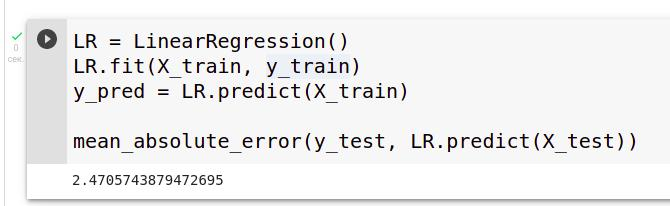
\includegraphics[]{my_result.jpg}
	\end{center}
	\caption{Демонстрация моего результата}
\end{figure}